\section{轴的计算与校核}
\subsection{高速轴设计计算}
\subsubsection{计算得到的相关运动参数}
    \[
        转速 n = 975r/min;功率 P =10.97kW;轴的转矩T=1.07\times 10^5 N\cdot mm
    \]
\subsubsection{轴的材料选择确定许用应力}
    选择$40Cr$调质,硬度为$280HBS$,许用弯曲应力为$[\sigma]=60MPa$
\subsubsection{按扭转强度概略计算轴的最小直径}
    材料的$C:107\sim 98$
    \[
        d \geq C\times \sqrt[3]{\frac{P}{n}}=(107\sim 98)\times \sqrt[3]{\frac{10.97}{975}}=(23.98\sim 21.96)mm
        \]

    最小轴端界面开一个键槽,将轴径增大$7\%$,得出轴的最小直径$(26.429\sim 23.5)mm$,查的标准轴的直径$d=32mm$。
\begin{figure}[h]
    \centering
    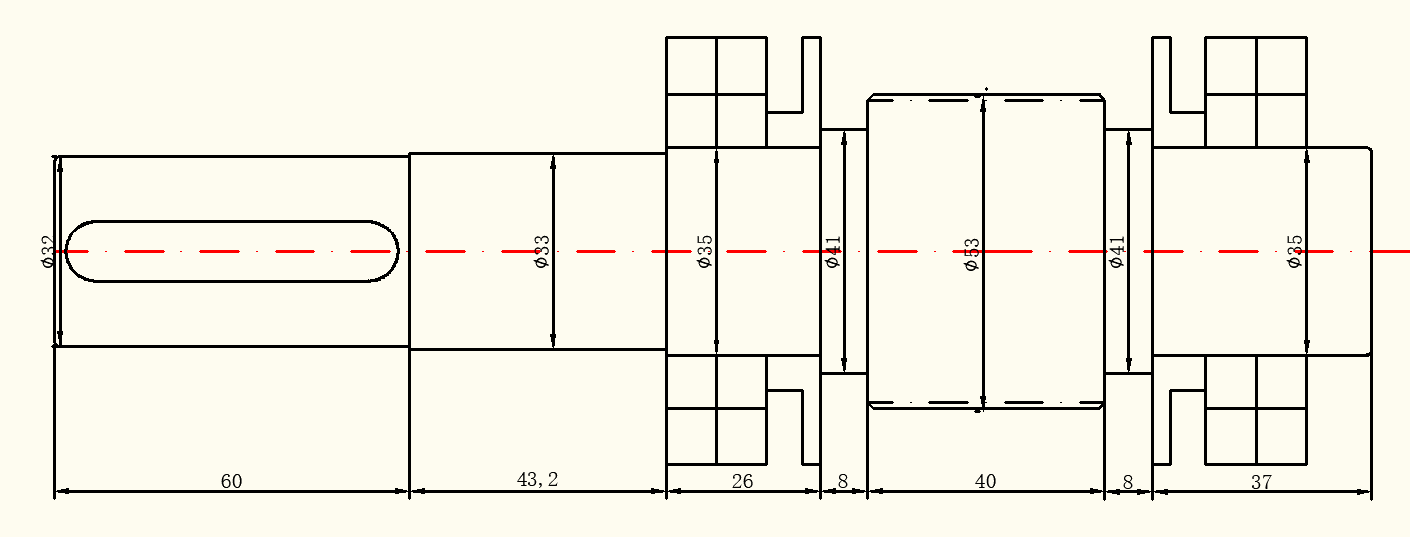
\includegraphics[scale=0.5]{graphic/5-1.png}
    \caption{轴的结构设计图}
\end{figure}

(1)高速轴与联轴器配合

标准轴径为$d_{12}=32mm$,$l_{12}$略大于联轴器轴孔长度$L=60mm$,取$l_{12}=64mm$。

选择弹性套柱销联轴器$LT6$,公称转矩$355N\cdot mm$,许用转速$3800r/min$。

选用普通平键,A型键,$b\times h=10\times 8$,取键长$L=56mm$。

(2)初步选择滚动轴承

因承受径向载荷的作用,选用角接触球轴承,选择型号$7207AC$ ,尺寸为$b\times D \times B=35\times 72 \times 17$,定位肩高度$41mm$。

轴承采用挡油环进行轴向固定。取$d_{45}=d_{46}=41mm$。

(3)由于齿轮的直径较小,为了保证齿轮轮体的强度,将齿轮和轴做为齿轮轴。因此上$l_{56}=45mm,d{56}=54mm$

(4)使用凸缘式轴承盖,轴承盖厚度$e=dn=1.2\times 6mm$,垫片厚度$\delta t=2mm$,使轴承盖便于拆卸,保证轴承盖外端面与联轴器有一定距离$K=24$,因此$L_{23}=43.2mm$,

(5)保证旋转零件端面至箱体内壁的距离$a=10\sim 15mm$,现取$L_{78}=37mm$。

确定的轴的尺寸见下表

\begin{tabular}{|c|c|c|c|c|c|c|c|}
    \hline
    直径& $32$&$33$&$35$&$41$&$53$&$41$&$35$\\
    \hline
    长度&$60$&$43.2$&$26$&$8$&$40$&$8$&$37$\\
    \hline
\end{tabular}

\subsubsection{受力分析与校核}
\begin{figure}[h]
    \centering
    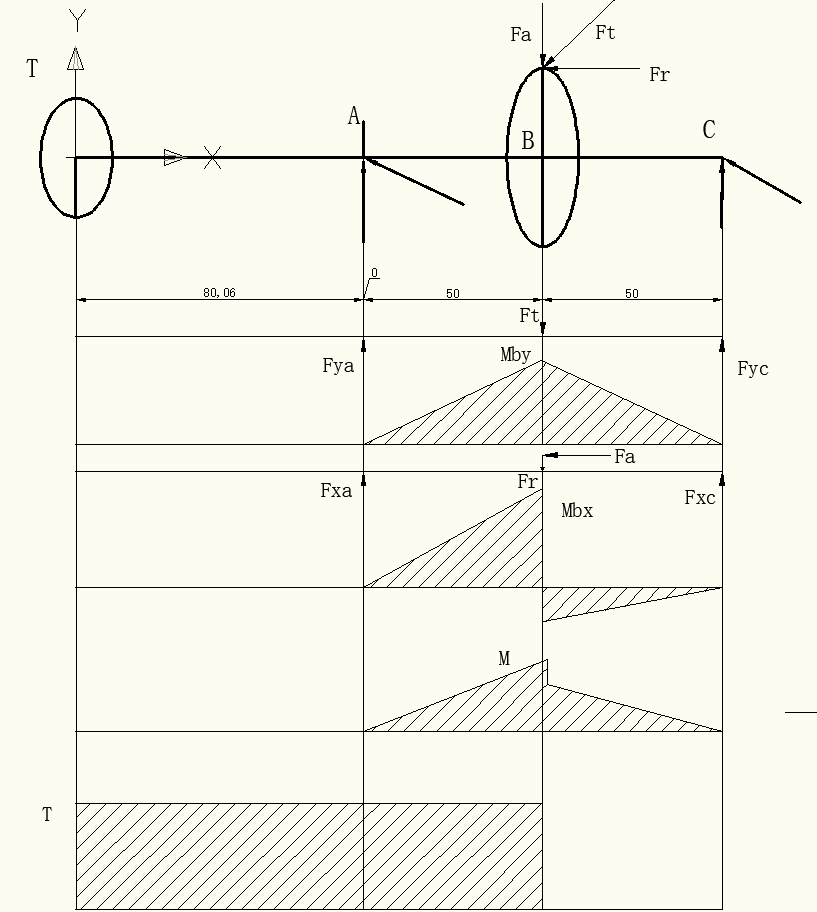
\includegraphics[scale=0.7]{graphic/5-2.png}
    \caption{高速轴的受力分析简图}
    \label{img1}
\end{figure}

(1)小齿轮受力情况如下:
\begin{align}
    \text{圆周力}       \qquad   F_{t1}=2\times \frac{T}{d_1}=4323.94N \\
    \text{径向力} \qquad          F_{r1}=F_{t1}\frac{tan\alpha_n}{cos \beta}=1630.50N\\
    \text{轴向力}       \qquad          F_{a1}=F_{t1}\times tan\beta =1171.23\\
    \text{电动机转矩} \qquad\qquad      T=107.45N\cdot m
\end{align}

齿宽中点距左支点距离 $L_2 =50mm$

齿宽中点距右支点距离 $L_3 =50mm$

(2)计算轴的支反力

垂直面支反力
\begin{align*}
    F_{ya}=\frac{F_{t1}L_3}{L_2+L_3}=2161.97N\\
    F_{yc}=\frac{F_{t1}L_2}{L_2+L_3}=2161.97N
\end{align*}

水平面支反力
\begin{align*}
    F_{xa}=\frac{F_{a1}{\frac{d_1}{2}}+F_{r1}L_3}{L_2+L_3} =1106.47N \\
    F_{xc}=\frac{F_{r1}{L_2}-F_{a1}\frac{d_1}{2}}{L_2+L_3}=524.2N
\end{align*}

(3)计算轴的弯矩,绘制弯矩图如\ref{img1}

截面$B$处的垂直弯矩
\[
    M_{by}=F_{ya}L_2=108098.5N\cdot mm
\]
截面$B$处的水平弯矩
\[
    M_{bx1}=F_{xa}L_2=55337N\cdot mm
\]
\[
    M_{bx2}=F_{xc}L_3=-26210N\cdot mm
\]
截面处的合成弯矩
\begin{align*}
    M_1=\sqrt{M_{by}^2+M_{bx1}^2}=121439.16N\cdot mm\\
    M_2=\sqrt{M_{by}^2+M_{bx2}^2}=111230.62N\cdot mm
\end{align*}

(4)画出电机施加的转矩图

(5)校核轴上承受最大弯矩和转矩的截面,即截面$B$

材料的抗弯截面系数
\[
    W=\frac{\pi d_1^2}{32}=12052mm^3
\]
弯曲应力
\[
    \sigma = \frac{M_1}{W} =10.76MPa
\]
抗扭截面系数
\[
    W_T=\frac{\pi d_1^2}{16}=24105mm^3
\]
切应力
\[
    \tau = \frac{T}{W}_T =4.46MPa
\]
按转矩脉动变化$\alpha =0.6$
\[
    \sigma_e =\sqrt{\sigma^2+4\times (\alpha \times \tau)^2}=11.65MPa
\]
材料选用$40Cr$调质,抗拉极限强度$\sigma_B=734MPa$,轴的许用弯曲应力$[\sigma_{-1b}=60MPa]$,因此设计的轴有足够的强度。   



\subsection{低速轴设计计算}
\subsubsection{计算得到的相关运动参数}
\[
        转速 n = 203.15r/min;功率 P =10.53kW;轴的转矩T=4.95\times 10^5 N\cdot mm
\]
\subsubsection{轴的材料选择确定的许用应力}
    选择$45$钢调质,硬度为$280HBS$,许用弯曲应力为$[\sigma]=60MPa$
\subsubsection{按扭转强度概略计算轴的最小直径}
材料的$C:118\sim 107$
    \[
        d \geq C\times \sqrt[3]{\frac{P}{n}}=(118\sim 107)\times \sqrt[3]{\frac{10.53}{203.15}}=(44\sim 40)mm
    \]
    最小轴端界面开一个键槽,将轴径增大$7\%$,得出轴的最小直径$(47.08\sim 42.8)mm$,查的标准轴的直径$d=50mm$。
\begin{figure}[h]
    \centering
    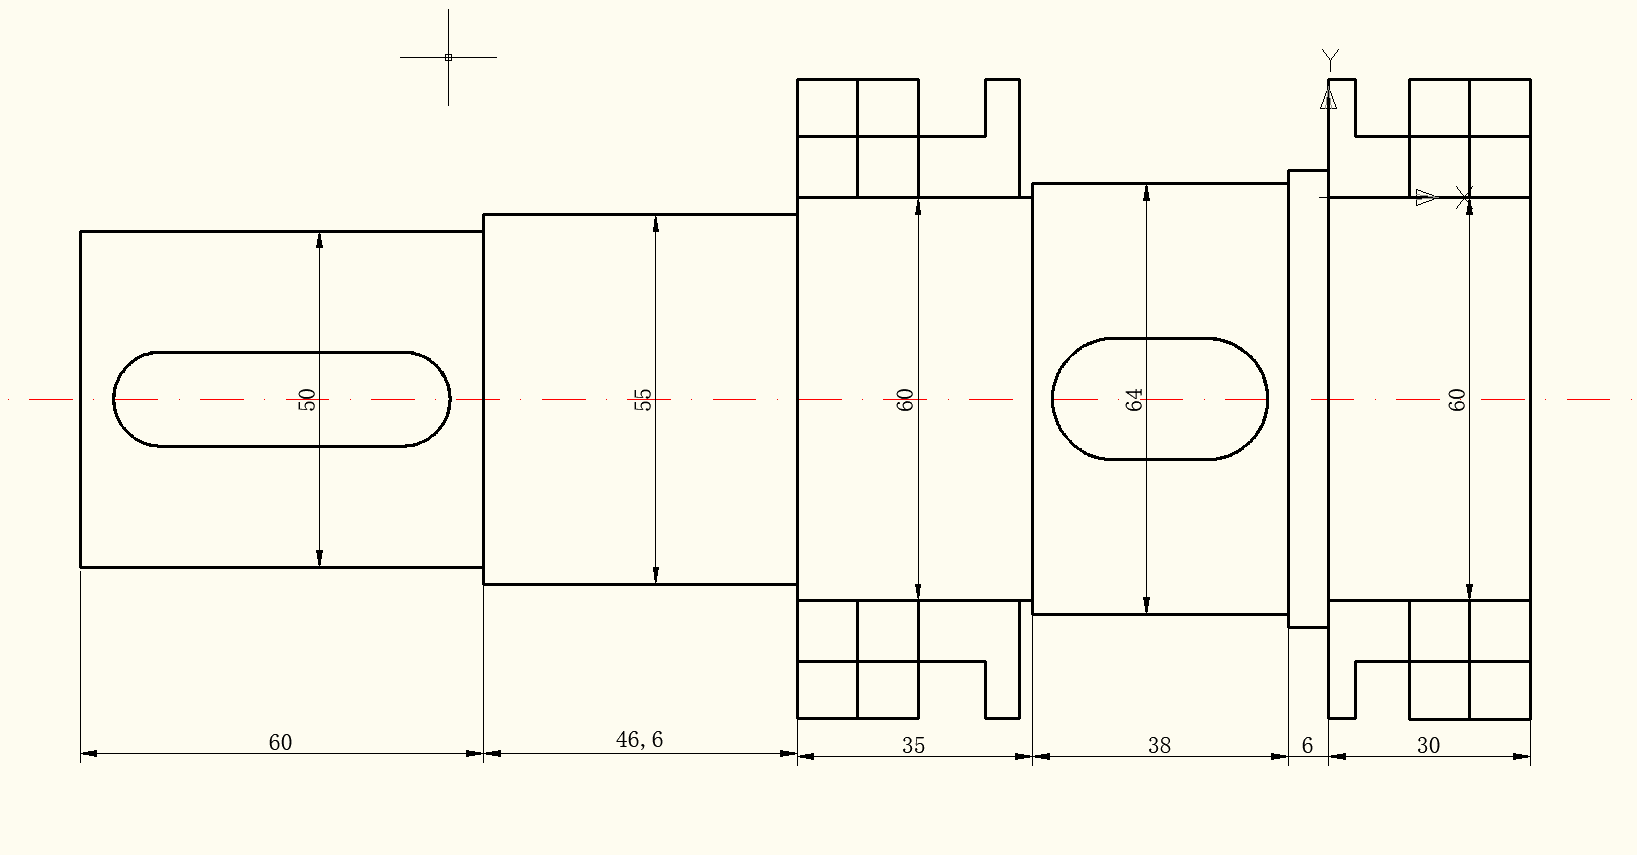
\includegraphics[scale=0.4]{graphic/5-3.png}
    \caption{轴的结构设计图}
\end{figure}

(1)低速轴与外齿轮配合

标准轴径为$d_{12}=50mm$,$l_{12}$略大于齿轮齿宽$L=40mm$,取$l_{12}=60mm$。

选用普通平键,$A$型键,$b\times h=14\times 9$,取键长$L=40mm$。

(2)初步选择滚动轴承

因承受径向载荷的作用,选用角接触球轴承,选择型号$7012AC$ ,尺寸为$b\times D \times B=60\times 95 \times 18$,定位肩高度$68mm$。

轴承采用挡油环进行轴向固定。取$d_{56}=68mm$。

(3)取安装齿轮处的轴段的直径$d_{45} = 64mm$;齿轮的左端与左轴承之间采用套筒定位。已知大齿轮轮毂的宽度为$b=40 mm$,为了使套筒端面可靠地压紧齿轮,此轴段应略短于轮毂宽度,故取$l_{45} = 38 mm$。

(4)使用凸缘式轴承盖,轴承盖厚度$e=dn=1.2\times 8mm$,垫片厚度$\Delta t=2mm$,使轴承盖便于拆卸,保证轴承盖外端面与联轴器有一定距离$K=24$,因此$L_{23}=46.6mm$。

(5)保证旋转零件端面至箱体内壁的距离$a=10\sim 15mm$,现取$L_{78}=30mm$。

确定的轴的尺寸见下表

\begin{tabular}{|c|c|c|c|c|c|c|}
    \hline
    直径& $50$&$55$&$60$&$64$&$68$&$60$\\
    \hline
    长度&$60$&$46.6$&$35$&$38$&$6$&$30$\\
    \hline
\end{tabular}
\subsubsection{受力分析与校核}
(1)小齿轮受力情况如下:
\begin{align}
    \text{圆周力}       \qquad   F_{t2}=2\times \frac{T}{d_2}=4119.22N \\
    \text{径向力} \qquad          F_{r2}=F_{t2}\frac{tan\alpha_n}{cos \beta}=1553.3N\\
    \text{轴向力}       \qquad          F_{a2}=F_{t2}\times tan\beta =1115.77\\
    \text{电动机转矩} \qquad\qquad      T=495.13N\cdot m
\end{align}

齿宽中点距左支点距离 $L_2 =42mm$

齿宽中点距右支点距离 $L_3 =46mm$

\begin{figure}[h]
    \centering
    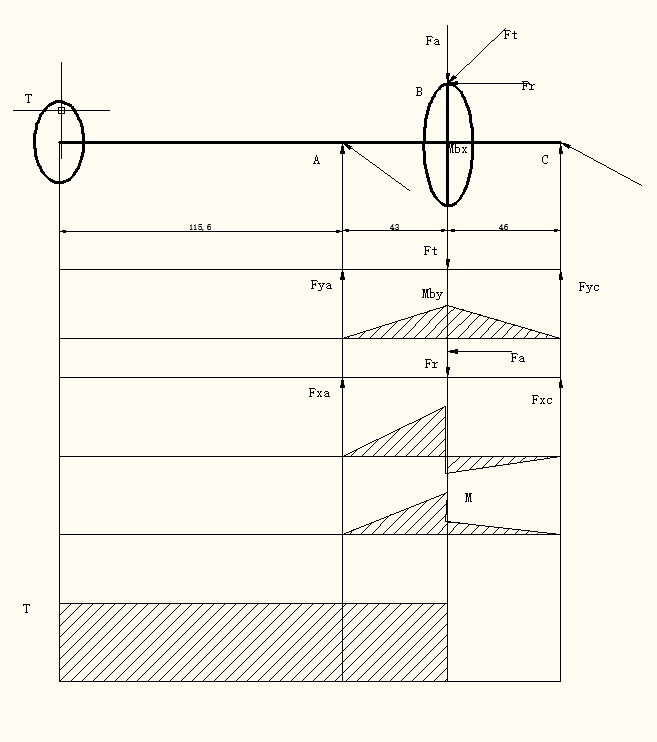
\includegraphics[scale=0.8]{graphic/5-4.png}
    \caption{高速轴的受力分析简图}
    \label{img2}
\end{figure}

(2)计算轴的支反力

垂直面支反力
\begin{align*}
    F_{ya}=\frac{F_{t2}L_3}{L_2+L_3}=2129.04N\\
    F_{yc}=\frac{F_{t2}L_2}{L_2+L_3}=1990.18N
\end{align*}

水平面支反力
\begin{align*}
    F_{xa}=\frac{F_{a2}{\frac{d_2}{2}}+F_{r2}L_3}{L_2+L_3} =1997.77N \\
    F_{xc}=\frac{F_{r2}{L_2}-F_{a2}\frac{d_2}{2}}{L_2+L_3}=-444.47N
\end{align*}

(3)计算轴的弯矩,绘制弯矩图如\ref{img2}

截面$B$处的垂直弯矩
\[
    M_{by1}=F_{ya}L_2=91548.72N\cdot mm
\]
\[
    M_{by2}=F_{ya}L_3=91548.28N\cdot mm
\]
截面$B$处的水平弯矩
\[
    M_{bx1}=F_{xa}L_2=85904.11N\cdot mm
\]
\[
    M_{bx2}=F_{xc}L_3=20445.62N\cdot mm
\]
截面处的合成弯矩
\begin{align*}
    M_1=\sqrt{M_{by1}^2+M_{bx1}^2}=125541.56N\cdot mm\\
    M_2=\sqrt{M_{by2}^2+M_{bx2}^2}=93803.58N\cdot mm
\end{align*}

(4)画出电机施加的转矩图

(5)校核轴上承受最大弯矩和转矩的截面,即截面$B$

材料的抗弯截面系数
\[
    W=\frac{\pi d_1^2}{32}=25735.93mm^3
\]
弯曲应力
\[
    \sigma = \frac{M_1}{W} =4.88MPa
\]
抗扭截面系数
\[
    W_T=\frac{\pi d_1^2}{16}=51471.85mm^3
\]
切应力
\[
    \tau = \frac{T}{W}_T =9.61MPa
\]
按转矩脉动变化$\alpha =0.6$
\[
    \sigma_e =\sqrt{\sigma^2+4\times (\alpha \times \tau)^2}=12.52MPa
\]
材料选用$45$钢调质,抗拉极限强度$\sigma_B=600MPa$,轴的许用弯曲应力$[\sigma_{-1b}=60MPa]$,因此设计的轴有足够的强度。   
